\chapter{Background and Literature Review}
\section{ The National Electricity Market }
\subsection{ Operation of the Spot Market }
\subsection{ Operation of the Ancillary Service Market }
\subsection{ Pre-dispatch Forecast Process }
Within the NEM, a pre-dispatch process is performed by Australian Energy Market Operator to ensure that market participants have sufficient pricing information to make informed and timely business decisions. In turn, this information provides the market with the information it needs to provide security of supply.  AEMO publishes somewhat limited information during pre-dispatch, however in evaluating battery storage this is vital to ensuring appropriate state of charge for future energy arbitrage opportunities. AEMO processes 2 different pre-dispatch to forecast price, 5 minute and 30 minute.
\subsubsection{P5 Region Solution}
The 5-minute Pre-dispatch cycle runs every 5-minutes to produce a dispatch and pricing schedule to a 5-minute resolution covering the next hour, for a total of twelve periods. It is key to note these prices represent forecasts for 5 minute dispatch prices rather than trading prices. Figure \ref{fig:p5_process_1} shows predicted dispatch price via the P5 Region Solution within the trading interval of 12:30:00pm, on the 1st of January, 2018, in South Australia. 
\begin{figure}[!h]
\centering
\includegraphics[width=0.8\textwidth]{Pictures/Chapter2/P5_Process.png}
\caption{P5 Predispatch Process - South Australia, Trading Interval 01/01/2018 12:30:00 PM}
\label{fig:p5_process_1}
\end{figure}
As seen in Figure \ref{fig:p5_process_1}, the P5 Region solution runs each 5 minutes and accuracy converges as forecast period approaches the dispatch interval. Although the forecast may not appear very accurate, Figure \ref{fig:p5_process_2} shows the P5 Price forecast elapsed for a full 24 hrs, clearly showing price follows the trend set by the forecast. 
\begin{figure}[!h]
\centering
\includegraphics[width=1\textwidth]{Pictures/Chapter2/P5_Process_2.png}
\caption{P5 Pre-dispatch Process - South Australia, 01/01/2018 - 02/01/2018}
\label{fig:p5_process_2}
\end{figure}
To date, no peer-reviewed academic analysis has been performed on the accuracy of the P5 Price forecast. The fundamental justification is most likely the shear size of the data set \textit{(For each year there are over 6 million rows of data for the 5 NEM jurisdictions)}. However, \parencite{AEMCMarch2017} provides insight into the magnitude of P5 Price forecast error by NEM region for the period 1 September 2015 to 8 March 2017, as shown in Figure \ref{fig:p5_aemc}. 
\begin{figure}[!htb]
\centering
\includegraphics[width=1\textwidth]{Pictures/Chapter2/AEMC_P5_Error.PNG}
\caption{AEMC 2017: Magnitude of Forecast Error Varies by Region.}
\label{fig:p5_aemc}
\end{figure}
\parencite{AEMCMarch2017} highlights 3 key elements regarding the P5 price forecast; accuracy improves as dispatch nears, the distribution is relatively symmetric with no apparent bias to overvaluing or under-valuing price and finally South Australia appears to have the greatest price discrepancy in absolute terms, however this is likely to be due to the underlying average price of the state being higher.


\subsubsection{P30 Predispatch Price}

To ensure it reliability of the P30 Predispatch Price forecast, the 48 half hours supply schedules of the following trading day need to be submitted by the generators by 12.30pm on the day before dispatch \parencite{Predispatch}. The expected wholesale electricity prices for the next day are then produced by matching these supply schedules with the demand forecasts, ancillary service requirements, inter-regional and intra-regional limits, in addition to solar and wind energy forecasts. 


\tikzset{every picture/.style={line width=0.75pt}} %set default line width to 0.75pt        

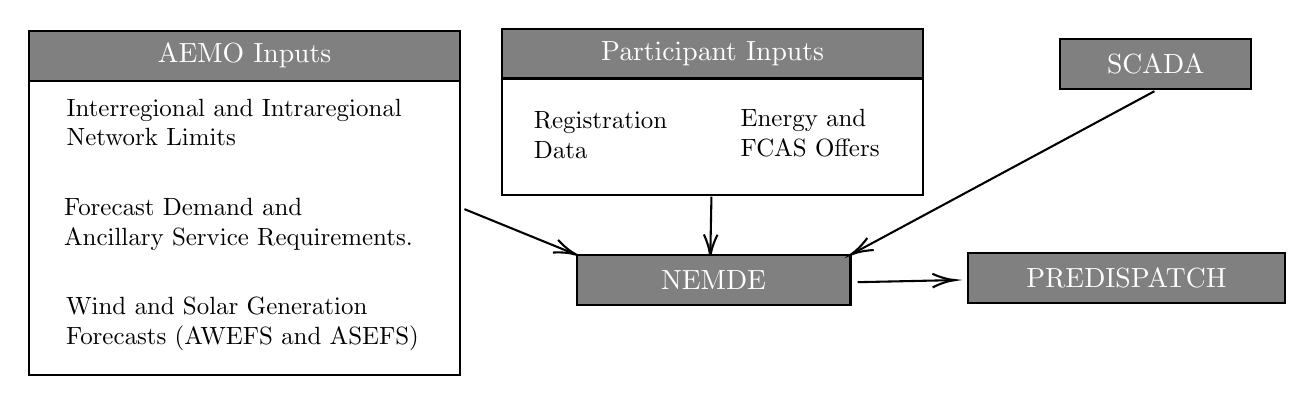
\begin{tikzpicture}[x=0.75pt,y=0.75pt,yscale=-1,xscale=1]
%uncomment if require: \path (0,191.0132598876953); %set diagram left start at 0, and has height of 191.0132598876953

%Straight Lines [id:da9177958313522097] 
\draw    (357.44,91.83) -- (356.91,119.02) ;
\draw [shift={(356.87,121.02)}, rotate = 271.13] [color={rgb, 255:red, 0; green, 0; blue, 0 }  ][line width=0.75]    (10.93,-3.29) .. controls (6.95,-1.4) and (3.31,-0.3) .. (0,0) .. controls (3.31,0.3) and (6.95,1.4) .. (10.93,3.29)   ;

%Straight Lines [id:da12798518797085823] 
\draw    (238.44,97.83) -- (290.59,119.07) ;
\draw [shift={(292.44,119.83)}, rotate = 202.17000000000002] [color={rgb, 255:red, 0; green, 0; blue, 0 }  ][line width=0.75]    (10.93,-3.29) .. controls (6.95,-1.4) and (3.31,-0.3) .. (0,0) .. controls (3.31,0.3) and (6.95,1.4) .. (10.93,3.29)   ;

%Shape: Rectangle [id:dp13477801690658042] 
\draw   (256.5,10.9) -- (459.5,10.9) -- (459.5,90.9) -- (256.5,90.9) -- cycle ;
%Shape: Rectangle [id:dp8582430372753662] 
\draw  [fill={rgb, 255:red, 128; green, 128; blue, 128 }  ,fill opacity=1 ] (256.5,10.9) -- (459.5,10.9) -- (459.5,34.9) -- (256.5,34.9) -- cycle ;
%Shape: Rectangle [id:dp5655505133083187] 
\draw   (28.5,11.9) -- (236.44,11.9) -- (236.44,177.9) -- (28.5,177.9) -- cycle ;
%Shape: Rectangle [id:dp5185219575052318] 
\draw  [fill={rgb, 255:red, 128; green, 128; blue, 128 }  ,fill opacity=1 ] (28.5,11.9) -- (236.44,11.9) -- (236.44,35.9) -- (28.5,35.9) -- cycle ;


%Shape: Rectangle [id:dp11057728244309994] 
\draw  [fill={rgb, 255:red, 128; green, 128; blue, 128 }  ,fill opacity=1 ] (292.44,119.83) -- (424.44,119.83) -- (424.44,143.83) -- (292.44,143.83) -- cycle ;
%Shape: Rectangle [id:dp07113446577922766] 
\draw  [fill={rgb, 255:red, 128; green, 128; blue, 128 }  ,fill opacity=1 ] (525.5,15.9) -- (617.44,15.9) -- (617.44,39.9) -- (525.5,39.9) -- cycle ;

%Straight Lines [id:da9707191163095252] 
\draw    (570.87,41.02) -- (426.2,118.88) ;
\draw [shift={(424.44,119.83)}, rotate = 331.71000000000004] [color={rgb, 255:red, 0; green, 0; blue, 0 }  ][line width=0.75]    (10.93,-3.29) .. controls (6.95,-1.4) and (3.31,-0.3) .. (0,0) .. controls (3.31,0.3) and (6.95,1.4) .. (10.93,3.29)   ;

%Shape: Rectangle [id:dp46501665361769806] 
\draw  [fill={rgb, 255:red, 128; green, 128; blue, 128 }  ,fill opacity=1 ] (480.87,118.83) -- (633.87,118.83) -- (633.87,142.83) -- (480.87,142.83) -- cycle ;
%Straight Lines [id:da4584246014213331] 
\draw    (427.87,133.02) -- (472.87,132.06) ;
\draw [shift={(474.87,132.02)}, rotate = 538.78] [color={rgb, 255:red, 0; green, 0; blue, 0 }  ][line width=0.75]    (10.93,-3.29) .. controls (6.95,-1.4) and (3.31,-0.3) .. (0,0) .. controls (3.31,0.3) and (6.95,1.4) .. (10.93,3.29)   ;


% Text Node
\draw (358,22.9) node [color={rgb, 255:red, 255; green, 255; blue, 255 }  ,opacity=1 ] [align=left] {Participant Inputs};
% Text Node
\draw (304,62) node [scale=0.9] [align=left] {Registration\\Data};
% Text Node
\draw (405,61) node [scale=0.9] [align=left] {Energy and\\FCAS Offers};
% Text Node
\draw (132.47,23.9) node [color={rgb, 255:red, 255; green, 255; blue, 255 }  ,opacity=1 ] [align=left] {AEMO Inputs};
% Text Node
\draw (129.53,105) node [scale=0.9] [align=left] {Forecast Demand and \\Ancillary Service Requirements.};
% Text Node
\draw (127.5,56) node [scale=0.9] [align=left] {Interregional and Intraregional \\Network Limits};
% Text Node
\draw (131.5,153) node [scale=0.9] [align=left] {Wind and Solar Generation \\Forecasts (AWEFS and ASEFS)};
% Text Node
\draw (571.47,27.9) node [color={rgb, 255:red, 255; green, 255; blue, 255 }  ,opacity=1 ] [align=left] {SCADA};
% Text Node
\draw (358.44,131.83) node [color={rgb, 255:red, 255; green, 255; blue, 255 }  ,opacity=1 ] [align=left] {NEMDE};
% Text Node
\draw (557.37,130.83) node [color={rgb, 255:red, 255; green, 255; blue, 255 }  ,opacity=1 ] [align=left] {PREDISPATCH};


\end{tikzpicture}

\caption{AEMO Pre-dispatch Process.}
\label{diagram:predispatch_process}


Those prices are also known as pre-dispatch prices for the next day. The granularity of the predispatch prices are given in 5 minute and 30 minute intervals, the 5 minute and 30 minute predispatch forecasts respectively. The 5-minute predispatch forecast is extends 1 hour whilst the 30-minute predispatch extend until the end of the following trading day with variable time horizon spanning between 28 intervals (14 hrs) up to 79 intervals (39.5 hrs)
\parencite{Predispatch}. \\
Pre-dispatch pricing does vary materially from actual pricing. In March 2017, the AEMC quantitatively highlighted how predispatch accuracy increases as the dispatch period nears.
\begin{table}[!h]
\begin{tabular}{l|c|c|c|}
\cline{2-4}
                                   & \multicolumn{3}{l|}{\cellcolor[HTML]{EFEFEF}\textbf{Percentage of Accurately Predicted High Prices}}                                    \\ \cline{2-4} 
                                   & \multicolumn{1}{l|}{\textit{One hour out}} & \multicolumn{1}{l|}{\textit{Four hours out}} & \multicolumn{1}{l|}{\textit{Ten hours out}} \\ \hline
\multicolumn{1}{|l|}{\textbf{NSW}} & 77\%                                       & 66\%                                         & 59\%                                        \\ \hline
\multicolumn{1}{|l|}{\textbf{QLD}} & 73\%                                       & 61\%                                         & 54\%                                        \\ \hline
\multicolumn{1}{|l|}{\textbf{SA}}  & 61\%                                       & 46\%                                         & 39\%                                        \\ \hline
\multicolumn{1}{|l|}{\textbf{TAS}} & 47\%                                       & 38\%                                         & 33\%                                        \\ \hline
\multicolumn{1}{|l|}{\textbf{VIC}} & 52\%                                       & 52\%                                         & 45\%                                        \\ \hline
\end{tabular}
\end{table}
Justification of tasmania \url{https://www.economicregulator.tas.gov.au/Documents/Energy%20in%20Tasmania%202016-17%20Report.pdf }

\section{ Utility Battery Energy Storage Dispatch Models }
\subsection{ Energy Arbitrage }
\subsection{ Energy Arbitrage with Imperfect Foresight }
\subsection{ Energy Arbitrage with Co-optimised with FCAS Participation }
\subsection{ Performance of Existing Utility Battery Energy Storage Plants in the NEM }
\subsubsection{ Hornsdale Power Reserve }
\subsubsection{ Gannawarra Energy Storage System }
\subsubsection{ Lake Bonney Precinct Battery Energy Storage System }
\section{ NEM Changing Generation Mix  }
\subsection{ Overview }
\subsection{ Modelling Techniques }
\section{ Policy and Investment Supporting Utility Storage   }
\subsection{ Australian Context }
\subsection{ Examples Abroad }

\section*{Citation examples}
\begin{enumerate}
\item A citation command in parentheses: \parencite{Smith:2012qr}.
\item A citation command for use in the flow of text: As \textcite{Smith:2013jd} said \dots
\item A citation command which automatically switches style depending on location and the option setting in the package declaration (see line 12 in the LaTeX source code). In this case, it produces a citation in parentheses: \autocite{Other:2014ab}.
\end{enumerate}